% !TEX program = pdflatex
\documentclass[aspectratio=169, 11pt]{beamer}

% ── Theme & Colors ──
\usetheme{Madrid}
\usecolortheme{whale}
\definecolor{deepblue}{RGB}{0, 51, 102}
\definecolor{accentred}{RGB}{180, 30, 30}
\definecolor{softgreen}{RGB}{34, 139, 34}
\definecolor{lightgray}{RGB}{240, 240, 240}
\definecolor{hlrow}{RGB}{220, 235, 255}

\setbeamercolor{frametitle}{bg=deepblue, fg=white}
\setbeamercolor{title}{bg=deepblue, fg=white}
\setbeamercolor{block title}{bg=deepblue, fg=white}
\setbeamercolor{block body}{bg=lightgray, fg=black}
\setbeamercolor{block title alerted}{bg=accentred, fg=white}
\setbeamercolor{block body alerted}{bg=lightgray, fg=black}
\setbeamercolor{block title example}{bg=softgreen, fg=white}
\setbeamercolor{block body example}{bg=lightgray, fg=black}
\setbeamercolor{item}{fg=deepblue}
\setbeamertemplate{navigation symbols}{}
\setbeamertemplate{footline}[frame number]

% ── Packages ──
\usepackage{amsmath, amssymb, mathtools}
\usepackage{booktabs}
\usepackage{array}
\usepackage{tikz}
\usetikzlibrary{arrows.meta, positioning, shapes.geometric, calc, decorations.pathmorphing, fit, backgrounds}
\usepackage{pgfplots}
\pgfplotsset{compat=1.18}
\usepackage{colortbl}
\usepackage{multirow}
\usepackage{graphicx}
\usepackage{hyperref}
\usepackage{adjustbox}
\usepackage{tabularx}
\usepackage{xcolor}
\usepackage{pifont}

\newcommand{\rmark}{\rho_{k,j}^{(l)}}

% ── Title Page ──
\title[Feature Entanglement in VFL]{Jacobian-Based Feature Entanglement Analysis\\for Vertical Federated Learning Unlearning}
\subtitle{A Comprehensive Technical Walkthrough}
\author{VFU-ML Project}
\date{\today}
\institute{CSE 472 --- Machine Learning}

\begin{document}

% ================================================================
%  TITLE
% ================================================================
\begin{frame}
  \titlepage
\end{frame}

% ================================================================
%  OUTLINE
% ================================================================
\begin{frame}{Outline}
  \tableofcontents
\end{frame}

% ================================================================
\section{Executive Summary}
% ================================================================

\begin{frame}{Executive Summary}
  \begin{block}{The Core Idea}
    Use the \textbf{Jacobian matrix} and \textbf{Singular Value Decomposition (SVD)} to measure how strongly one party's features influence another party's model in \textbf{Vertical Federated Learning (VFL)}.
  \end{block}
  \vspace{0.3cm}
  \begin{columns}[T]
    \begin{column}{0.48\textwidth}
      \textbf{Novelty:}
      \begin{itemize}
        \item No existing paper implements this \emph{exact} method
        \item Uniquely combines:\\
              \textcolor{deepblue}{Cross-party Jacobian SVD}\\
              \textcolor{deepblue}{+ VFL unlearning context}\\
              \textcolor{deepblue}{+ Pre-unlearning diagnostic}
      \end{itemize}
    \end{column}
    \begin{column}{0.48\textwidth}
      \textbf{Grounding:}
      \begin{itemize}
        \item Every \emph{individual} component has strong prior work:
        \begin{itemize}
          \item Jacobian sensitivity analysis
          \item SVD-based low-rank approx.
          \item Feature entanglement in unlearning
        \end{itemize}
      \end{itemize}
    \end{column}
  \end{columns}
\end{frame}

\begin{frame}{What Problem Does This Solve?}
  \begin{center}
    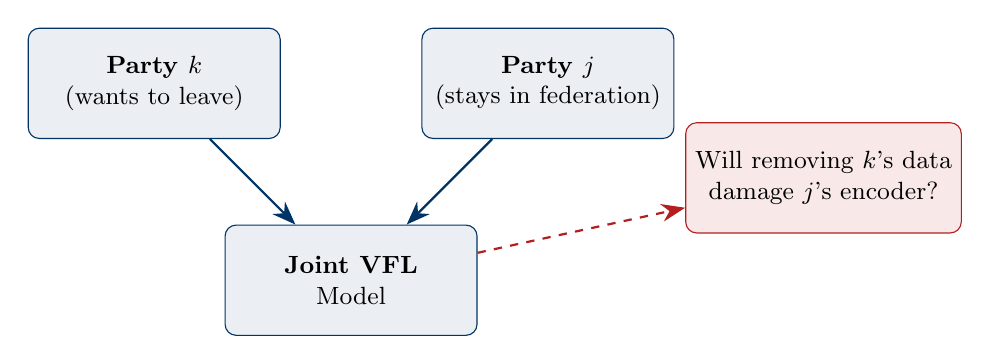
\begin{tikzpicture}[
      box/.style={rectangle, draw=deepblue, fill=deepblue!8, rounded corners=4pt,
                  minimum width=3.2cm, minimum height=1.4cm, align=center, font=\small},
      arr/.style={-{Stealth[length=3mm]}, thick, deepblue},
      warn/.style={rectangle, draw=accentred, fill=accentred!10, rounded corners=4pt,
                   minimum width=3.5cm, minimum height=1.4cm, align=center, font=\small}
    ]
      \node[box] (pk) at (0,0) {\textbf{Party $k$}\\(wants to leave)};
      \node[box] (pj) at (5,0) {\textbf{Party $j$}\\(stays in federation)};
      \node[box] (model) at (2.5,-2.5) {\textbf{Joint VFL}\\Model};
      \draw[arr] (pk) -- (model);
      \draw[arr] (pj) -- (model);
      \node[warn] (q) at (8.5, -1.2) {Will removing $k$'s data\\damage $j$'s encoder?};
      \draw[-{Stealth[length=3mm]}, thick, accentred, dashed] (model) -- (q);
    \end{tikzpicture}
  \end{center}
  \vspace{0.2cm}
  \begin{alertblock}{The Gap}
    Current VFL unlearning methods operate \textbf{blindly} — they remove data but give \textbf{no warning} about collateral damage to remaining parties.
  \end{alertblock}
\end{frame}

% ================================================================
\section{Background: VFL \& Unlearning}
% ================================================================

\begin{frame}{Vertical Federated Learning (VFL) Architecture}
  \begin{center}
    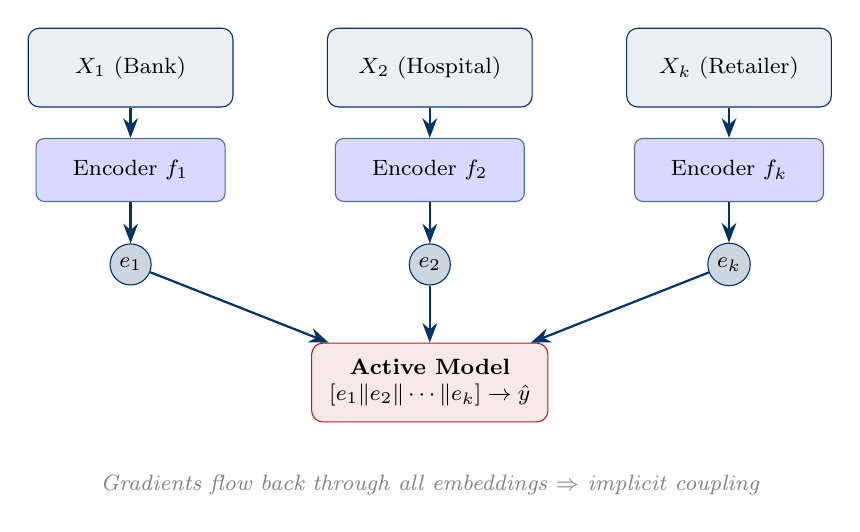
\begin{tikzpicture}[
      party/.style={rectangle, draw=deepblue, fill=deepblue!8, rounded corners=4pt,
                    minimum width=2.6cm, minimum height=1.0cm, align=center, font=\footnotesize},
      enc/.style={rectangle, draw=deepblue!70, fill=blue!15, rounded corners=3pt,
                  minimum width=2.4cm, minimum height=0.8cm, align=center, font=\footnotesize},
      emb/.style={circle, draw=deepblue, fill=deepblue!20, inner sep=2pt, font=\footnotesize},
      active/.style={rectangle, draw=accentred, fill=accentred!10, rounded corners=4pt,
                     minimum width=3.0cm, minimum height=1.0cm, align=center, font=\footnotesize},
      arr/.style={-{Stealth[length=2.5mm]}, thick, deepblue}
    ]
      \node[party]  (p1) at (0,   2.5) {$X_1$ (Bank)};
      \node[party]  (p2) at (3.8, 2.5) {$X_2$ (Hospital)};
      \node[party]  (p3) at (7.6, 2.5) {$X_k$ (Retailer)};

      \node[enc] (e1) at (0,   1.2) {Encoder $f_1$};
      \node[enc] (e2) at (3.8, 1.2) {Encoder $f_2$};
      \node[enc] (e3) at (7.6, 1.2) {Encoder $f_k$};

      \draw[arr] (p1) -- (e1);
      \draw[arr] (p2) -- (e2);
      \draw[arr] (p3) -- (e3);

      \node[emb] (em1) at (0,   0) {$e_1$};
      \node[emb] (em2) at (3.8, 0) {$e_2$};
      \node[emb] (em3) at (7.6, 0) {$e_k$};

      \draw[arr] (e1) -- (em1);
      \draw[arr] (e2) -- (em2);
      \draw[arr] (e3) -- (em3);

      \node[active] (agg) at (3.8, -1.5) {\textbf{Active Model}\\$[e_1 \| e_2 \| \cdots \| e_k] \to \hat{y}$};
      \draw[arr] (em1) -- (agg);
      \draw[arr] (em2) -- (agg);
      \draw[arr] (em3) -- (agg);

      \node[font=\footnotesize\itshape, text=gray] at (3.8, -2.8) {Gradients flow back through all embeddings $\Rightarrow$ implicit coupling};
    \end{tikzpicture}
  \end{center}
\end{frame}

\begin{frame}{Why Unlearning Causes Cross-Party Damage}
  \begin{columns}[T]
    \begin{column}{0.55\textwidth}
      \textbf{Three mechanisms of implicit coupling:}
      \begin{enumerate}
        \item \textbf{Shared Loss:} All encoders optimize the same objective $\Rightarrow$ gradients couple representations
        \item \textbf{Feature Correlation:} If $X_k$ and $X_j$ are statistically correlated (e.g., income \& spending), encoder $f_j$ exploits regularities involving $X_k$
        \item \textbf{Active Model Adaptation:} The top model learns joint patterns from concatenated embeddings
      \end{enumerate}
    \end{column}
    \begin{column}{0.42\textwidth}
      \begin{exampleblock}{Empirical Evidence (LASER-VFL)}
        When a client's feature block is removed, model accuracy drops by \textbf{$>$18\%} even for clients whose features \emph{remain available}.
        \vspace{0.15cm}\\
        {\footnotesize \textit{— LASER-VFL, ICLR 2025}}
      \end{exampleblock}
    \end{column}
  \end{columns}
\end{frame}

% ================================================================
\section{Literature Survey}
% ================================================================

\begin{frame}{Related Work: Landscape Overview}
  \begin{center}
    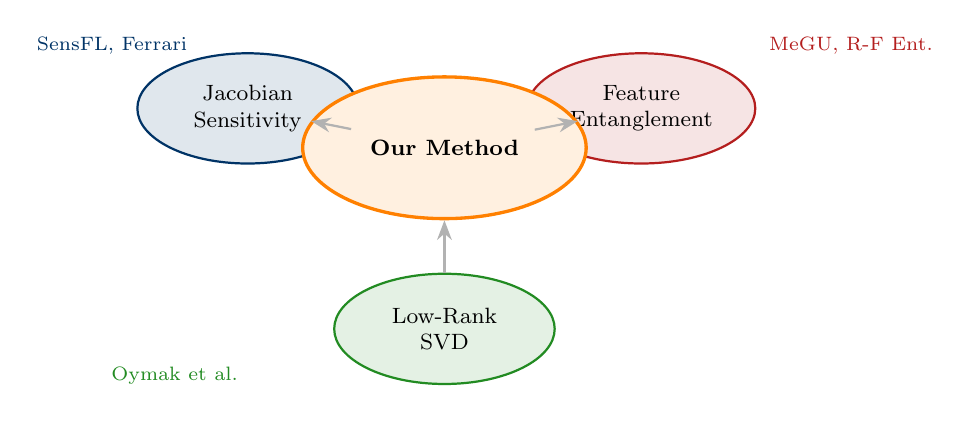
\begin{tikzpicture}[
      bub/.style={ellipse, draw=#1, fill=#1!12, align=center, font=\footnotesize,
                  minimum width=2.8cm, minimum height=1.4cm, thick},
      arr/.style={-{Stealth[length=2.5mm]}, thick, gray!60}
    ]
      \node[bub=deepblue]  (jac)  at (0, 0)     {Jacobian\\Sensitivity};
      \node[bub=accentred]  (ent)  at (5, 0)     {Feature\\Entanglement};
      \node[bub=softgreen] (svd)  at (2.5, -2.8) {Low-Rank\\SVD};
      \node[bub=orange, minimum width=3.6cm, minimum height=1.8cm, very thick]
            (ours) at (2.5, -0.5) {\textbf{Our Method}};

      \draw[arr] (jac) -- (ours);
      \draw[arr] (ent) -- (ours);
      \draw[arr] (svd) -- (ours);

      \node[font=\scriptsize, text=deepblue, anchor=west] at (-2.8, 0.8) {SensFL, Ferrari};
      \node[font=\scriptsize, text=accentred, anchor=west] at (6.5, 0.8) {MeGU, R-F Ent.};
      \node[font=\scriptsize, text=softgreen, anchor=east] at (0, -3.4) {Oymak et al.};
    \end{tikzpicture}
  \end{center}
  \vspace{0.1cm}
  \begin{center}
    \textit{Each component has strong prior work; the \textbf{integration} is novel.}
  \end{center}
\end{frame}

\begin{frame}{Detailed Literature Comparison}
  \begin{adjustbox}{max width=\textwidth}
    \renewcommand{\arraystretch}{1.25}
    \begin{tabular}{>{\bfseries\footnotesize}p{2.2cm} >{\footnotesize}c >{\footnotesize}p{4.0cm} >{\footnotesize}p{5.5cm}}
      \toprule
      \textbf{Paper} & \textbf{Year} & \textbf{What It Does} & \textbf{How It Differs from Ours} \\
      \midrule
      \rowcolor{hlrow}
      SensFL & 2025 & Jacobian $L_2$ norm $\|{\partial e_n}/{\partial x_n}\|_2$ for embedding sensitivity & Same-party sensitivity only; privacy defense, not cross-party influence \\
      Ferrari & 2024 & Feature sensitivity via Lipschitz continuity & Horizontal FL; measures output sensitivity, not embedding dependency \\
      \rowcolor{hlrow}
      MeGU & 2026 & Feature-pattern entanglement via MLLM similarity & Centralized unlearning; no Jacobian SVD \\
      Retain-Forget Ent. & 2026 & Correlated-feature damage during unlearning & Augmented Lagrangian + Wasserstein-2, not Jacobian \\
      \rowcolor{hlrow}
      Oymak et al. & 2019 & Low-rank Jacobian: ``information'' vs ``nuisance'' spaces & Theoretical foundation; applied to generalization, not unlearning \\
      Certified VFU & 2025 & First certified VFL unlearning; notes cascading impacts & Confidence matrix updates, not Jacobian analysis \\
      \rowcolor{hlrow}
      LASER-VFL & 2025 & Missing features $\Rightarrow$ accuracy drop & Validates concern empirically, no diagnostic tool \\
      \bottomrule
    \end{tabular}
  \end{adjustbox}
\end{frame}

\begin{frame}{The Key Gap}
  \begin{center}
    \renewcommand{\arraystretch}{1.3}
    \begin{tabular}{>{\footnotesize}p{5.5cm} >{\footnotesize}c >{\footnotesize}c >{\footnotesize}c}
      \toprule
      & \textbf{Jacobian} & \textbf{Cross-Party} & \textbf{VFL Unlearning} \\
      \midrule
      SensFL           & \textcolor{softgreen}{\checkmark} & \textcolor{accentred}{\ding{55}} & \textcolor{accentred}{\ding{55}} \\
      Ferrari          & \textcolor{accentred}{\ding{55}} & \textcolor{accentred}{\ding{55}} & \textcolor{softgreen}{\checkmark} \\
      MeGU             & \textcolor{accentred}{\ding{55}} & \textcolor{accentred}{\ding{55}} & \textcolor{softgreen}{\checkmark} \\
      Certified VFU    & \textcolor{accentred}{\ding{55}} & \textcolor{softgreen}{\checkmark} & \textcolor{softgreen}{\checkmark} \\
      \midrule
      \rowcolor{deepblue!15}
      \textbf{Proposed Method} & \textcolor{softgreen}{\checkmark} & \textcolor{softgreen}{\checkmark} & \textcolor{softgreen}{\checkmark} \\
      \bottomrule
    \end{tabular}
  \end{center}
  \vspace{0.3cm}
  \begin{block}{Unique Combination}
    \centering
    \textbf{Cross-party} $+$ \textbf{Jacobian SVD} $+$ \textbf{VFL Unlearning} $+$ \textbf{Pre-unlearning Diagnostic}
  \end{block}
\end{frame}

% ================================================================
\section{Theoretical Foundation}
% ================================================================

\begin{frame}{Why the Jacobian? --- Sensitivity as a Matrix}
  \begin{block}{Definition}
    The Jacobian of function $f: \mathbb{R}^n \to \mathbb{R}^m$ is the $m \times n$ matrix of all first-order partial derivatives:
    \[
    J = \frac{\partial f}{\partial x} = \begin{bmatrix}
      \frac{\partial f_1}{\partial x_1} & \cdots & \frac{\partial f_1}{\partial x_n} \\
      \vdots & \ddots & \vdots \\
      \frac{\partial f_m}{\partial x_1} & \cdots & \frac{\partial f_m}{\partial x_n}
    \end{bmatrix}
    \]
  \end{block}
  \vspace{0.2cm}
  \textbf{Interpretation:} Entry $J_{ij}$ tells us how much output $f_i$ changes when input $x_j$ changes by a tiny amount.

  \vspace{0.2cm}
  \textbf{In VFL:} $J = \dfrac{\partial h_j^{(l)}}{\partial X_k}$ maps how party $k$'s input features affect party $j$'s hidden activations.
\end{frame}

\begin{frame}{The Low-Rank Property of Neural Network Jacobians}
  \begin{columns}[T]
    \begin{column}{0.52\textwidth}
      \begin{block}{Key Finding (Oymak et al., NeurIPS 2019)}
        Neural network Jacobians are \textbf{naturally low-rank}: a few large singular values dominate; most are near zero.
      \end{block}
      \vspace{0.2cm}
      The spectrum decomposes into:
      \begin{itemize}
        \item \textcolor{deepblue}{\textbf{Information Space}} — top singular values capturing meaningful data relationships
        \item \textcolor{gray}{\textbf{Nuisance Space}} — small singular values capturing noise
      \end{itemize}
      \vspace{0.2cm}
      {\footnotesize Recent work confirms this holds across architectures and deepens during training.}
    \end{column}
    \begin{column}{0.45\textwidth}
      \begin{center}
        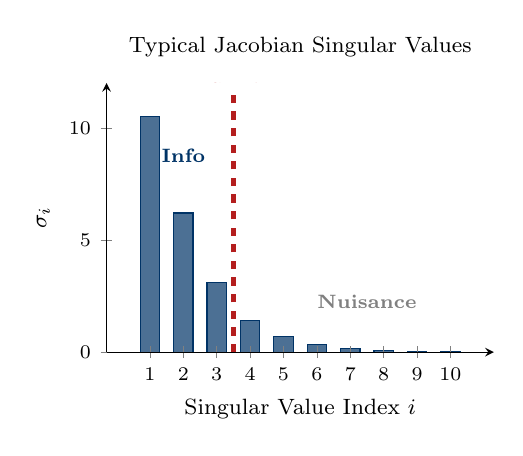
\begin{tikzpicture}
          \begin{axis}[
            width=6.5cm, height=5cm,
            ybar,
            bar width=7pt,
            xlabel={Singular Value Index $i$},
            ylabel={$\sigma_i$},
            ymin=0, ymax=12,
            xmin=0.5, xmax=10.5,
            xtick={1,...,10},
            title={\footnotesize Typical Jacobian Singular Values},
            title style={font=\footnotesize},
            label style={font=\footnotesize},
            tick label style={font=\scriptsize},
            axis lines=left,
            enlarge x limits=0.08,
            area style,
          ]
            \addplot[fill=deepblue!70, draw=deepblue] coordinates {
              (1,10.5) (2,6.2) (3,3.1) (4,1.4) (5,0.7)
              (6,0.35) (7,0.18) (8,0.09) (9,0.04) (10,0.02)
            };
            \draw[accentred, ultra thick, dashed] (axis cs:3.5,0) -- (axis cs:3.5,11.5)
              node[above, font=\scriptsize, text=accentred] {rank $r$};
            \node[font=\scriptsize, text=deepblue, anchor=south] at (axis cs:2,8) {\textbf{Info}};
            \node[font=\scriptsize, text=gray, anchor=south] at (axis cs:7.5,1.5) {\textbf{Nuisance}};
          \end{axis}
        \end{tikzpicture}
      \end{center}
    \end{column}
  \end{columns}
\end{frame}

\begin{frame}{SensFL: Jacobian Sensitivity in VFL}
  \begin{block}{SensFL Formulation (CMES 2025)}
    For each client $n$, compute Jacobian norm:
    \[
    J_n = \left\| \frac{\partial e_n}{\partial x_n} \right\|_2
    \]
    Add as regularization $\Rightarrow$ reduces information content of embeddings $\Rightarrow$ defends against reconstruction attacks while maintaining accuracy ($<5\%$ drop).
  \end{block}

  \vspace{0.3cm}
  \begin{columns}
    \begin{column}{0.48\textwidth}
      \textcolor{softgreen}{\textbf{What SensFL validates:}}
      \begin{itemize}
        \item Jacobian captures meaningful feature-to-representation dependencies
        \item Practical in VFL settings
      \end{itemize}
    \end{column}
    \begin{column}{0.48\textwidth}
      \textcolor{accentred}{\textbf{What SensFL misses:}}
      \begin{itemize}
        \item Only measures \emph{same-party} sensitivity ($\partial e_n / \partial x_n$)
        \item Does not address \emph{cross-party} influence ($\partial h_j / \partial X_k$)
      \end{itemize}
    \end{column}
  \end{columns}
\end{frame}

\begin{frame}{Why Cross-Party Extension Is Needed}
  \begin{center}
    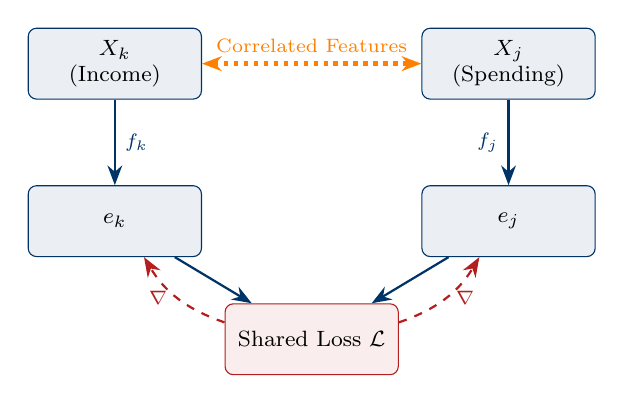
\begin{tikzpicture}[
      box/.style={rectangle, draw=deepblue, fill=deepblue!8, rounded corners=3pt,
                  minimum width=2.2cm, minimum height=0.9cm, align=center, font=\footnotesize},
      arr/.style={-{Stealth[length=2.5mm]}, thick},
    ]
      \node[box] (xk) at (0, 2) {$X_k$\\(Income)};
      \node[box] (xj) at (5, 2) {$X_j$\\(Spending)};
      \node[box] (ek) at (0, 0) {$e_k$};
      \node[box] (ej) at (5, 0) {$e_j$};
      \node[box, draw=accentred, fill=accentred!8] (loss) at (2.5, -1.5) {Shared Loss $\mathcal{L}$};

      \draw[arr, deepblue] (xk) -- (ek) node[midway, right, font=\scriptsize] {$f_k$};
      \draw[arr, deepblue] (xj) -- (ej) node[midway, left, font=\scriptsize]  {$f_j$};
      \draw[arr, deepblue] (ek) -- (loss);
      \draw[arr, deepblue] (ej) -- (loss);

      \draw[arr, accentred, dashed, thick] (loss) to[bend left=20] node[left, font=\scriptsize, text=accentred] {$\nabla$} (ek);
      \draw[arr, accentred, dashed, thick] (loss) to[bend right=20] node[right, font=\scriptsize, text=accentred] {$\nabla$} (ej);

      \draw[{Stealth[length=2.5mm]}-{Stealth[length=2.5mm]}, ultra thick, orange, dotted]
        (xk) -- (xj) node[midway, above, font=\scriptsize, text=orange] {Correlated Features};
    \end{tikzpicture}
  \end{center}
  \vspace{0.2cm}
  SensFL measures: $\partial e_k / \partial X_k$ \quad (how my features affect \emph{my} embedding)

  \textbf{We need:} $\partial h_j^{(l)} / \partial X_k$ \quad (how party $k$'s features affect party \textbf{$j$'s} encoder)
\end{frame}

% ================================================================
\section{Proposed Method: Step-by-Step}
% ================================================================

\begin{frame}{Method Overview}
  \begin{center}
    \begin{tikzpicture}[
      step/.style={rectangle, draw=deepblue, fill=deepblue!10, rounded corners=5pt,
                   minimum width=3.0cm, minimum height=1.0cm, align=center, font=\footnotesize\bfseries},
      arr/.style={-{Stealth[length=3mm]}, very thick, deepblue},
    ]
      \node[step] (s1) at (0,0)   {Step 1\\Cross-Party\\Jacobian};
      \node[step] (s2) at (3.5,0) {Step 2\\SVD \& $\rho$\\Metric};
      \node[step] (s3) at (7,0)   {Step 3\\Low-Rank\\Approximation};
      \node[step] (s4) at (10.5,0){Step 4\\Layer\\Aggregation};
      \node[step, draw=accentred, fill=accentred!10] (s5) at (13.5,0) {Step 5\\Classify\\Influence};

      \draw[arr] (s1) -- (s2);
      \draw[arr] (s2) -- (s3);
      \draw[arr] (s3) -- (s4);
      \draw[arr] (s4) -- (s5);
    \end{tikzpicture}
  \end{center}
  \vspace{0.3cm}
  \textbf{Goal:} Before unlearning party $k$'s features, \emph{predict} whether party $j$'s encoder will be harmed.

  \vspace{0.2cm}
  \textbf{Core Idea:} Measure how strongly $X_k$ influences $h_j^{(l)}$ via the cross-party Jacobian, then classify the risk level.
\end{frame}

\begin{frame}{Step 1: Compute the Cross-Party Jacobian}
  \begin{block}{Formulation}
    At each layer $l$ of party $j$'s model, compute:
    \[
    J^{(l)}_{k \to j} = \frac{\partial h_j^{(l)}}{\partial X_k}
    \quad \in \mathbb{R}^{\dim(h_j^{(l)}) \times \dim(X_k)}
    \]
  \end{block}

  \vspace{0.2cm}
  \begin{columns}[T]
    \begin{column}{0.55\textwidth}
      \textbf{What each entry means:}\\
      $J^{(l)}_{ij}$ = how much a small change in the $j$-th feature of party $k$ changes the $i$-th hidden activation of party $j$'s layer $l$.

      \vspace{0.2cm}
      \textbf{Analogy:} A \emph{sensitivity map} showing which of party $k$'s features party $j$'s encoder has learned to be sensitive to, even across organizational boundaries.
    \end{column}
    \begin{column}{0.42\textwidth}
      \begin{center}
        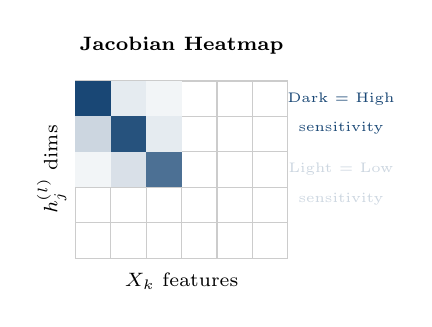
\begin{tikzpicture}[scale=0.75]
          \draw[step=0.6, gray!40, thin] (0,0) grid (3.6,3);
          \foreach \x/\y/\c in {0/2.4/0.9, 0.6/2.4/0.1, 1.2/2.4/0.05,
                                 0/1.8/0.2, 0.6/1.8/0.85, 1.2/1.8/0.1,
                                 0/1.2/0.05, 0.6/1.2/0.15, 1.2/1.2/0.7} {
            \pgfmathsetmacro{\intensity}{\c*100}
            \fill[deepblue!\intensity] (\x,\y) rectangle ++(0.6,0.6);
          }
          \node[font=\scriptsize, rotate=90] at (-0.4, 1.5) {$h_j^{(l)}$ dims};
          \node[font=\scriptsize] at (1.8, -0.4) {$X_k$ features};
          \node[font=\scriptsize\bfseries] at (1.8, 3.6) {Jacobian Heatmap};
          \node[font=\tiny] at (4.5, 2.7) {\textcolor{deepblue!90}{Dark = High}};
          \node[font=\tiny] at (4.5, 2.2) {\textcolor{deepblue!90}{sensitivity}};
          \node[font=\tiny] at (4.5, 1.5) {\textcolor{deepblue!20}{Light = Low}};
          \node[font=\tiny] at (4.5, 1.0) {\textcolor{deepblue!20}{sensitivity}};
        \end{tikzpicture}
      \end{center}
    \end{column}
  \end{columns}
\end{frame}

\begin{frame}{How Cross-Party Jacobian Arises in VFL}
  \begin{center}
    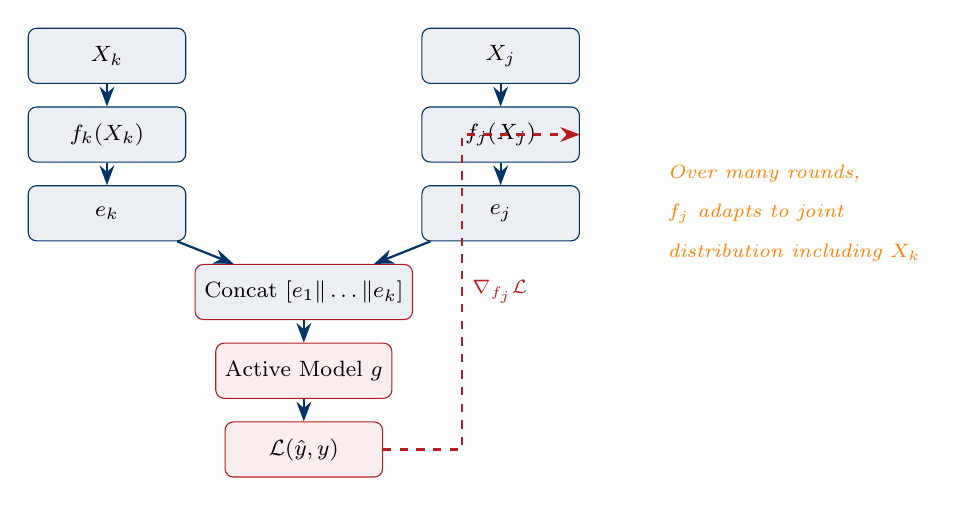
\begin{tikzpicture}[
      box/.style={rectangle, draw=deepblue, fill=deepblue!8, rounded corners=3pt,
                  minimum width=2cm, minimum height=0.7cm, align=center, font=\footnotesize},
      arr/.style={-{Stealth[length=2.5mm]}, thick, deepblue}
    ]
      \node[box] (xk)    at (0, 3)    {$X_k$};
      \node[box] (fk)    at (0, 2)    {$f_k(X_k)$};
      \node[box] (ek)    at (0, 1)    {$e_k$};
      \node[box, draw=accentred] (cat) at (2.5, 0) {Concat $[e_1\|\ldots\|e_k]$};
      \node[box, draw=accentred, fill=accentred!8] (top) at (2.5, -1) {Active Model $g$};
      \node[box, draw=accentred, fill=accentred!8] (loss) at (2.5, -2) {$\mathcal{L}(\hat{y}, y)$};

      \node[box] (xj)    at (5, 3)    {$X_j$};
      \node[box] (fj)    at (5, 2)    {$f_j(X_j)$};
      \node[box] (ej)    at (5, 1)    {$e_j$};

      \draw[arr] (xk)--(fk); \draw[arr] (fk)--(ek); \draw[arr] (ek)--(cat);
      \draw[arr] (xj)--(fj); \draw[arr] (fj)--(ej); \draw[arr] (ej)--(cat);
      \draw[arr] (cat)--(top); \draw[arr] (top)--(loss);

      \draw[-{Stealth[length=2.5mm]}, thick, accentred, dashed]
        (loss.east) -- ++(1,0) |- (fj.east)
        node[pos=0.25, right, font=\scriptsize, text=accentred] {$\nabla_{f_j}\mathcal{L}$};

      \node[font=\scriptsize\itshape, text=orange, anchor=west] at (7, 1.5) {Over many rounds,};
      \node[font=\scriptsize\itshape, text=orange, anchor=west] at (7, 1.0) {$f_j$ adapts to joint};
      \node[font=\scriptsize\itshape, text=orange, anchor=west] at (7, 0.5) {distribution including $X_k$};
    \end{tikzpicture}
  \end{center}
  \vspace{0.1cm}
  {\footnotesize Gradients from the shared loss flow back through all embeddings, creating \textbf{implicit coupling} — the Jacobian $\partial h_j^{(l)} / \partial X_k$ captures this.}
\end{frame}

\begin{frame}{Step 2: SVD and the $\rho$ Metric}
  \begin{block}{Singular Value Decomposition}
    \[
    \frac{\partial h_j^{(l)}}{\partial X_k} = U \Sigma V^T
    \quad \text{where } \Sigma = \text{diag}(\sigma_1 \geq \sigma_2 \geq \cdots \geq \sigma_r)
    \]
  \end{block}

  \begin{block}{The $\rho$ Metric (Feature Influence Concentration)}
    \[
    \boxed{\rho_{k,j}^{(l)} = \frac{\sigma_1}{\sqrt{\sum_i \sigma_i^2}} = \frac{\|\text{top singular value}\|_2}{\|\text{all singular values}\|_F}}
    \]
  \end{block}
  \vspace{0.2cm}
  \textbf{Range:} $\rho \in [0, 1]$
  \begin{itemize}
    \item $\rho \to 0$: Influence diffusely spread (many small singular values) — low risk
    \item $\rho \to 1$: Influence concentrated in one direction — \textbf{high risk}
  \end{itemize}
\end{frame}

\begin{frame}{Interpreting $\rho$: Visual Intuition}
  \begin{center}
    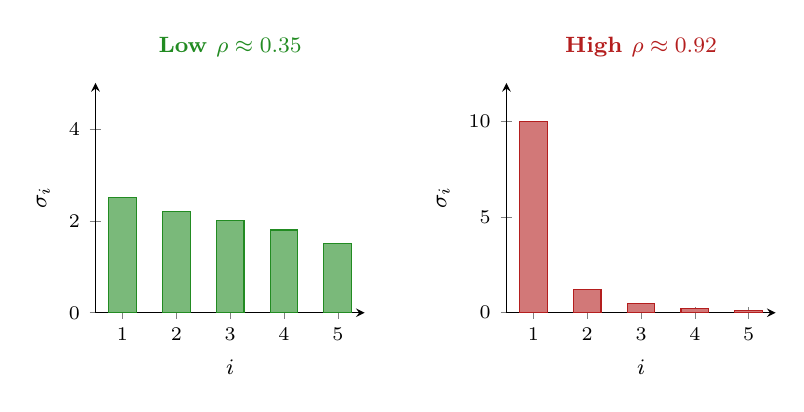
\begin{tikzpicture}
      \begin{axis}[
        name=low,
        width=5cm, height=4.5cm,
        ybar,
        bar width=10pt,
        xlabel={$i$},
        ylabel={$\sigma_i$},
        ymin=0, ymax=5,
        xmin=0.5, xmax=5.5,
        xtick={1,...,5},
        title={\footnotesize Low $\rho \approx 0.35$},
        title style={font=\footnotesize\bfseries, text=softgreen},
        label style={font=\footnotesize},
        tick label style={font=\scriptsize},
        axis lines=left,
      ]
        \addplot[fill=softgreen!60, draw=softgreen] coordinates {
          (1,2.5) (2,2.2) (3,2.0) (4,1.8) (5,1.5)
        };
      \end{axis}

      \begin{axis}[
        at={(low.east)}, anchor=west, xshift=1.8cm,
        width=5cm, height=4.5cm,
        ybar,
        bar width=10pt,
        xlabel={$i$},
        ylabel={$\sigma_i$},
        ymin=0, ymax=12,
        xmin=0.5, xmax=5.5,
        xtick={1,...,5},
        title={\footnotesize High $\rho \approx 0.92$},
        title style={font=\footnotesize\bfseries, text=accentred},
        label style={font=\footnotesize},
        tick label style={font=\scriptsize},
        axis lines=left,
      ]
        \addplot[fill=accentred!60, draw=accentred] coordinates {
          (1,10.0) (2,1.2) (3,0.5) (4,0.2) (5,0.1)
        };
      \end{axis}
    \end{tikzpicture}
  \end{center}
  \vspace{0.1cm}
  \begin{columns}
    \begin{column}{0.48\textwidth}
      \centering
      \textcolor{softgreen}{\textbf{Broad, shallow coupling}}\\
      {\footnotesize Encoder can adapt to removal\\$\Rightarrow$ Low unlearning risk}
    \end{column}
    \begin{column}{0.48\textwidth}
      \centering
      \textcolor{accentred}{\textbf{Concentrated, strong reliance}}\\
      {\footnotesize Encoder depends on one direction from $X_k$\\$\Rightarrow$ High unlearning risk}
    \end{column}
  \end{columns}
\end{frame}

\begin{frame}{Why Ratio, Not Absolute Magnitude?}
  \begin{center}
    \renewcommand{\arraystretch}{1.4}
    \begin{tabular}{>{\footnotesize}p{3.2cm} >{\footnotesize}c >{\footnotesize}c >{\footnotesize}p{5cm}}
      \toprule
      \textbf{Scenario} & $\|\Sigma\|_F$ & $\rho$ & \textbf{Implication} \\
      \midrule
      Large Jacobian,\newline even spread & High & \textcolor{softgreen}{Low} & Broad but shallow coupling — encoder \emph{can} adapt \\
      \rowcolor{hlrow}
      Large Jacobian,\newline concentrated & High & \textcolor{accentred}{High} & Encoder relies on one specific direction from $X_k$ — \textbf{brittle} \\
      Small Jacobian,\newline concentrated & Low & \textcolor{accentred}{High} & Even weak coupling is focused — still a directional dependency \\
      \rowcolor{hlrow}
      Small Jacobian,\newline even spread & Low & \textcolor{softgreen}{Low} & Minimal influence, spread thin — safest scenario \\
      \bottomrule
    \end{tabular}
  \end{center}
  \vspace{0.3cm}
  {\footnotesize The ratio \textbf{normalizes} by total influence, isolating the \emph{structural} nature of the dependency.}
\end{frame}

\begin{frame}{Step 3: Low-Rank Approximation for Efficiency}
  \begin{block}{Approximation}
    \[
    J \approx U_r \Sigma_r V_r^T
    \qquad \text{(keep only top-$r$ singular values/vectors)}
    \]
  \end{block}

  \vspace{0.2cm}
  \begin{columns}[T]
    \begin{column}{0.50\textwidth}
      \textbf{Memory Savings:}
      \begin{center}
        \renewcommand{\arraystretch}{1.3}
        \begin{tabular}{>{\footnotesize}l >{\footnotesize}c}
          \toprule
          \textbf{Representation} & \textbf{Memory} \\
          \midrule
          Full Jacobian & $O(d_1 \times d_2)$ \\
          \rowcolor{hlrow}
          Low-rank ($r$) & $O(r \times (d_1 + d_2))$ \\
          \bottomrule
        \end{tabular}
      \end{center}
      \vspace{0.2cm}
      {\footnotesize Example: $d_1 = 512$, $d_2 = 100$, $r = 10$\\
      Full: 51,200 \quad Low-rank: 6,120 \quad (\textbf{12$\times$ savings})}
    \end{column}
    \begin{column}{0.45\textwidth}
      \textbf{Why this works:}
      \begin{itemize}
        \item Neural network Jacobians are \emph{naturally} low-rank
        \item Small $r$ (5--20) captures dominant dependencies
        \item The $\rho$ metric only needs $\sigma_1$ and $\|\Sigma\|_F$ — perfectly captured by low-rank SVD
      \end{itemize}
    \end{column}
  \end{columns}
\end{frame}

\begin{frame}{Step 4: Aggregate Across Layers}
  \begin{block}{Layer Aggregation}
    For each (party $k$, party $j$) pair:
    \[
    \text{Influence}_{k \to j} = \text{median}\bigl(\rho_{k,j}^{(l)}\bigr) \quad \text{over all layers } l
    \]
  \end{block}

  \vspace{0.2cm}
  \textbf{Why median?}
  \begin{center}
    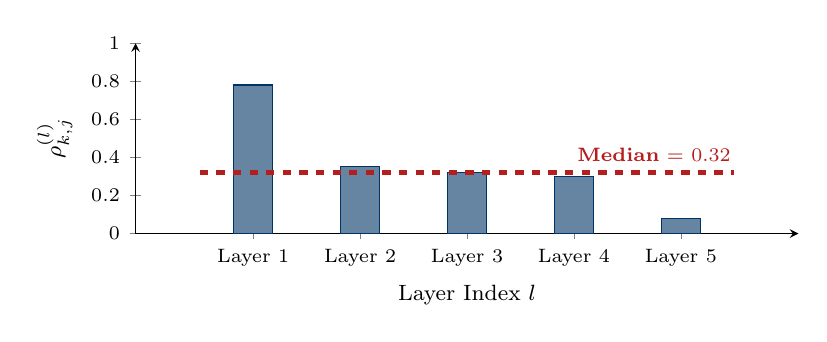
\begin{tikzpicture}
      \begin{axis}[
        width=10cm, height=4cm,
        ybar,
        bar width=14pt,
        xlabel={Layer Index $l$},
        ylabel={$\rho_{k,j}^{(l)}$},
        ymin=0, ymax=1,
        xmin=0.5, xmax=5.5,
        xtick={1,...,5},
        xticklabels={Layer 1, Layer 2, Layer 3, Layer 4, Layer 5},
        label style={font=\footnotesize},
        tick label style={font=\scriptsize},
        axis lines=left,
        enlarge x limits=0.12,
      ]
        \addplot[fill=deepblue!60, draw=deepblue] coordinates {
          (1,0.78) (2,0.35) (3,0.32) (4,0.30) (5,0.08)
        };
        \draw[accentred, ultra thick, dashed] (axis cs:0.5,0.32) -- (axis cs:5.5,0.32)
          node[pos=0.85, above, font=\scriptsize, text=accentred] {\textbf{Median} = 0.32};
      \end{axis}
    \end{tikzpicture}
  \end{center}
  {\footnotesize Layer 1 has anomalously high $\rho$ (direct feature contact); Layer 5 has low $\rho$ (vanishing gradients). Median captures the \textbf{typical} dependency.}
\end{frame}

\begin{frame}{Step 5: Classification Thresholds}
  \begin{center}
    \renewcommand{\arraystretch}{1.5}
    \begin{tabular}{>{\bfseries\small}l >{\small}c >{\small}p{4.5cm} >{\small}p{4.5cm}}
      \toprule
      \textbf{Level} & \textbf{Threshold} & \textbf{Interpretation} & \textbf{Recommended Action} \\
      \midrule
      \rowcolor{softgreen!15}
      Low & $\rho < 0.15$ & Minimal structured dependency on $X_k$ & Unlearning proceeds safely \\
      \rowcolor{orange!15}
      Medium & $0.15 \leq \rho < 0.40$ & Moderate coupling; some degradation possible & Monitor party $j$'s accuracy post-unlearning \\
      \rowcolor{accentred!15}
      High & $\rho \geq 0.40$ & Strong, concentrated dependency & \textbf{Warn:} party $j$ likely needs local retraining \\
      \bottomrule
    \end{tabular}
  \end{center}
  \vspace{0.3cm}
  \begin{alertblock}{Note}
    Thresholds are motivated by spectral theory ($\rho \geq 0.40$ means one direction captures $>$40\% of total variance) but require \textbf{empirical calibration} per dataset/architecture.
  \end{alertblock}
\end{frame}

\begin{frame}{Complete Pipeline Diagram}
  \begin{center}
    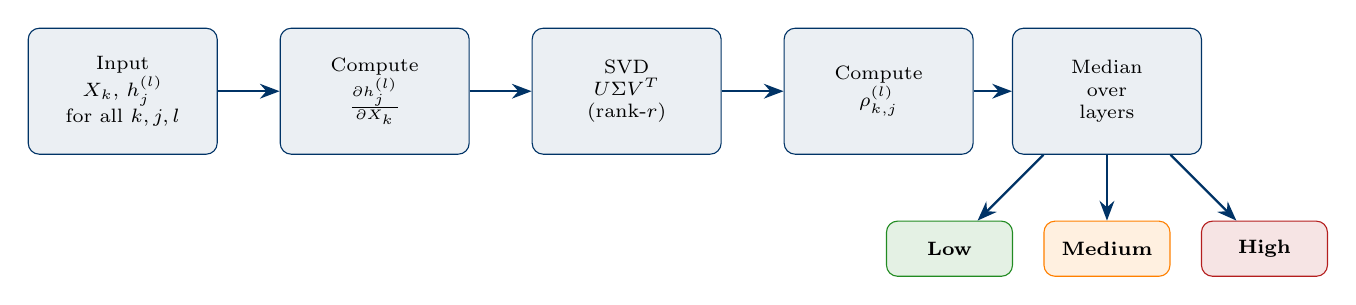
\begin{tikzpicture}[
      box/.style={rectangle, draw=deepblue, fill=deepblue!8, rounded corners=4pt,
                  minimum width=2.4cm, minimum height=1.6cm, align=center, font=\scriptsize},
      result/.style={rectangle, draw=#1, fill=#1!12, rounded corners=4pt,
                     minimum width=1.6cm, minimum height=0.7cm, align=center, font=\scriptsize\bfseries},
      arr/.style={-{Stealth[length=2.5mm]}, thick, deepblue}
    ]
      \node[box] (input) at (0,0) {Input\\$X_k$, $h_j^{(l)}$\\for all $k,j,l$};
      \node[box] (jac) at (3.2,0) {Compute\\$\frac{\partial h_j^{(l)}}{\partial X_k}$};
      \node[box] at (6.4,0) (svd) {SVD\\$U\Sigma V^T$\\(rank-$r$)};
      \node[box] at (9.6,0) (rho) {Compute\\$\rho_{k,j}^{(l)}$};
      \node[box] at (12.5,0) (agg) {Median\\over\\layers};

      \draw[arr] (input) -- (jac);
      \draw[arr] (jac) -- (svd);
      \draw[arr] (svd) -- (rho);
      \draw[arr] (rho) -- (agg);

      \node[result=softgreen]  (low)  at (10.5, -2) {Low};
      \node[result=orange]     (med)  at (12.5, -2) {Medium};
      \node[result=accentred]  (high) at (14.5, -2) {High};

      \draw[arr] (agg) -- (low);
      \draw[arr] (agg) -- (med);
      \draw[arr] (agg) -- (high);
    \end{tikzpicture}
  \end{center}
\end{frame}

% ================================================================
\section{Practical Utility}
% ================================================================

\begin{frame}{Why Is This Useful?}
  \begin{columns}[T]
    \begin{column}{0.32\textwidth}
      \begin{block}{Pre-Unlearning Diagnostic}
        Before executing unlearning, flag which remaining parties are at \textbf{risk of accuracy degradation}.
      \end{block}
    \end{column}
    \begin{column}{0.32\textwidth}
      \begin{block}{Informed Decisions}
        If high $\rho$ is detected, coordinator can \textbf{plan retraining proactively} rather than discovering damage post-hoc.
      \end{block}
    \end{column}
    \begin{column}{0.32\textwidth}
      \begin{block}{Threshold Automation}
        \textbf{Low:} auto-approve unlearning\\
        \textbf{Medium:} monitor\\
        \textbf{High:} human review + mitigation
      \end{block}
    \end{column}
  \end{columns}

  \vspace{0.4cm}
  \begin{exampleblock}{Current State of the Art}
    VFU-KD, VFU-GA, and Certified VFU all operate \textbf{blindly} w.r.t.\ cross-party feature entanglement. They remove data but provide \textbf{no warning} about collateral damage.
  \end{exampleblock}
\end{frame}

\begin{frame}{Validation from Adjacent Literature}
  \begin{center}
    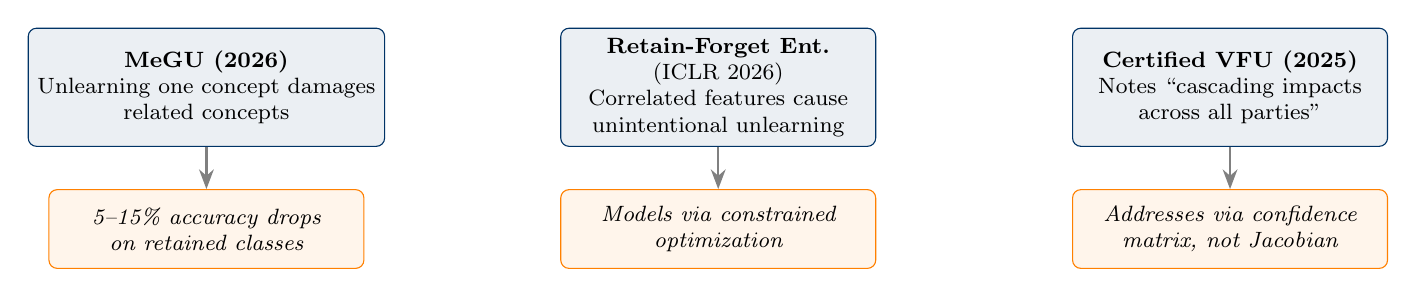
\begin{tikzpicture}[
      paper/.style={rectangle, draw=deepblue, fill=deepblue!8, rounded corners=3pt,
                    minimum width=4cm, minimum height=1.5cm, align=center, font=\footnotesize},
      finding/.style={rectangle, draw=orange, fill=orange!8, rounded corners=3pt,
                      minimum width=4cm, minimum height=1cm, align=center, font=\footnotesize\itshape},
      arr/.style={-{Stealth[length=2.5mm]}, thick, gray}
    ]
      \node[paper] (megu) at (0, 0) {\textbf{MeGU (2026)}\\Unlearning one concept damages\\related concepts};
      \node[finding] (mf) at (0, -1.8) {5--15\% accuracy drops\\on retained classes};

      \node[paper] (rf) at (6.5, 0) {\textbf{Retain-Forget Ent.}\\(ICLR 2026)\\Correlated features cause\\unintentional unlearning};
      \node[finding] (rff) at (6.5, -1.8) {Models via constrained\\optimization};

      \node[paper] (cvfu) at (13, 0) {\textbf{Certified VFU (2025)}\\Notes ``cascading impacts\\across all parties''};
      \node[finding] (cvf) at (13, -1.8) {Addresses via confidence\\matrix, not Jacobian};

      \draw[arr] (megu) -- (mf);
      \draw[arr] (rf) -- (rff);
      \draw[arr] (cvfu) -- (cvf);
    \end{tikzpicture}
  \end{center}
  \vspace{0.2cm}
  \begin{center}
    {\footnotesize All confirm the feature entanglement problem exists, but \textbf{none provide a Jacobian-based diagnostic}.}
  \end{center}
\end{frame}

% ================================================================
\section{Challenges \& Considerations}
% ================================================================

\begin{frame}{Challenge 1: Privacy Constraints}
  \begin{alertblock}{The Tension}
    Computing $\partial h_j^{(l)} / \partial X_k$ requires access to both party $j$'s model internals \textbf{and} party $k$'s input features — potentially violating VFL's privacy boundaries.
  \end{alertblock}
  \vspace{0.3cm}
  \textbf{Possible Mitigations:}
  \begin{enumerate}
    \item \textbf{Embedding-Level Computation:} Compute Jacobian only at the embedding level using stored embeddings at the active party (consistent with VFU-KD's assumptions)
    \item \textbf{Randomized SVD / Sketching:} Estimate the $\rho$ metric \emph{without} full Jacobian materialization
    \item \textbf{Trusted Third Party / Secure Computation:} MPC or TEE-based protocols to perform analysis without revealing raw data
  \end{enumerate}
\end{frame}

\begin{frame}{Challenge 2: Computational Cost}
  \begin{block}{Scaling}
    Cross-party Jacobians for all $(k, j)$ pairs across all layers:
    \[
    \text{Cost} = O\!\left(K^2 \times L \times r \times n\right)
    \]
    where $K$ = parties, $L$ = layers, $r$ = approx.\ rank, $n$ = samples.
  \end{block}
  \vspace{0.2cm}
  \begin{center}
    \renewcommand{\arraystretch}{1.3}
    \begin{tabular}{>{\footnotesize}l >{\footnotesize}c >{\footnotesize}c}
      \toprule
      \textbf{VFL Setting} & \textbf{Parties $K$} & \textbf{Feasibility} \\
      \midrule
      \rowcolor{softgreen!15}
      Typical (2--5 parties, simple arch.) & 2--5 & \textcolor{softgreen}{Manageable} \\
      \rowcolor{orange!15}
      Medium (5--10 parties, deep models) & 5--10 & \textcolor{orange}{Needs batch sampling} \\
      \rowcolor{accentred!15}
      Large (10+ parties, complex arch.) & 10+ & \textcolor{accentred}{Requires randomized estimation} \\
      \bottomrule
    \end{tabular}
  \end{center}
\end{frame}

\begin{frame}{Challenge 3: Threshold Calibration}
  Proposed thresholds ($0.15$, $0.40$) require empirical validation across:
  \vspace{0.2cm}
  \begin{center}
    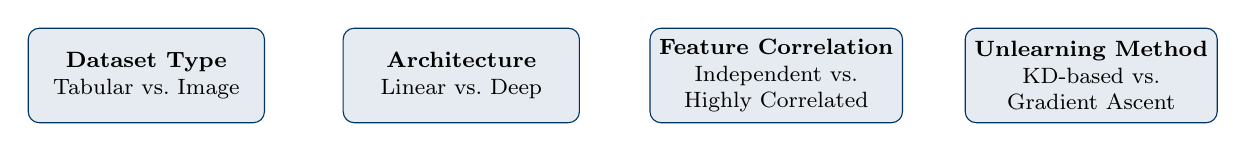
\begin{tikzpicture}[
      dim/.style={rectangle, draw=deepblue, fill=deepblue!10, rounded corners=4pt,
                  minimum width=3cm, minimum height=1.2cm, align=center, font=\footnotesize},
    ]
      \node[dim] (d1) at (0, 0)   {\textbf{Dataset Type}\\Tabular vs.\ Image};
      \node[dim] (d2) at (4, 0)   {\textbf{Architecture}\\Linear vs.\ Deep};
      \node[dim] (d3) at (8, 0)   {\textbf{Feature Correlation}\\Independent vs.\\ Highly Correlated};
      \node[dim] (d4) at (12, 0)  {\textbf{Unlearning Method}\\KD-based vs.\\ Gradient Ascent};
    \end{tikzpicture}
  \end{center}
  \vspace{0.3cm}
  \begin{exampleblock}{Insight from Ferrari}
    Lipschitz-continuity-based sensitivity thresholds vary \textbf{significantly} across domains $\Rightarrow$ $\rho$ thresholds likely need dataset-specific calibration too.
  \end{exampleblock}
\end{frame}

% ================================================================
\section{Research Contribution \& Positioning}
% ================================================================

\begin{frame}{Positioning as a Research Contribution}
  \begin{center}
    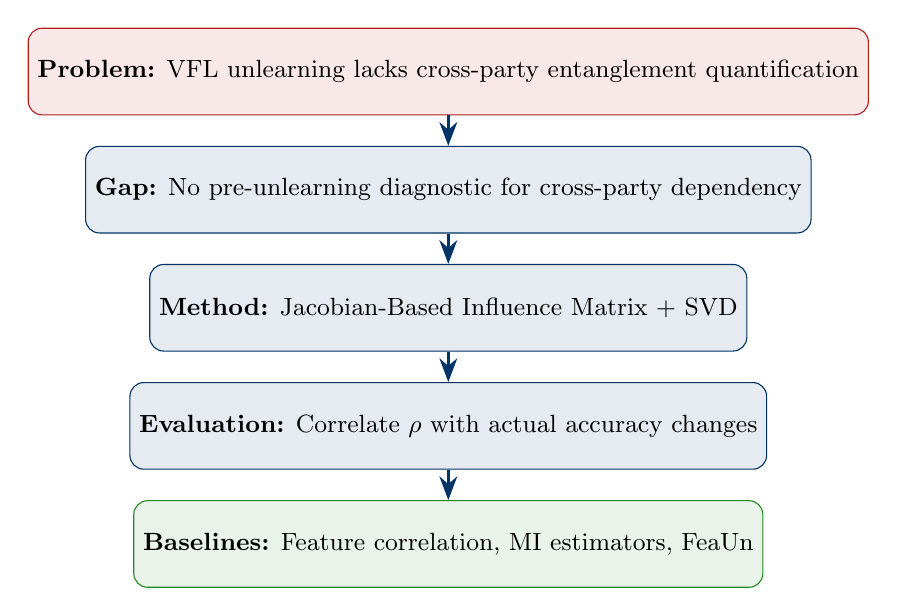
\begin{tikzpicture}[
      box/.style={rectangle, draw=deepblue, fill=deepblue!10, rounded corners=5pt,
                  minimum width=5cm, minimum height=1.1cm, align=center, font=\small},
      arr/.style={-{Stealth[length=3mm]}, very thick, deepblue}
    ]
      \node[box, draw=accentred, fill=accentred!10] (prob) at (0, 3) {\textbf{Problem:} VFL unlearning lacks cross-party entanglement quantification};
      \node[box] (gap) at (0, 1.5) {\textbf{Gap:} No pre-unlearning diagnostic for cross-party dependency};
      \node[box] (meth) at (0, 0) {\textbf{Method:} Jacobian-Based Influence Matrix + SVD};
      \node[box] (eval) at (0, -1.5) {\textbf{Evaluation:} Correlate $\rho$ with actual accuracy changes};
      \node[box, draw=softgreen, fill=softgreen!10] (base) at (0, -3) {\textbf{Baselines:} Feature correlation, MI estimators, FeaUn};

      \draw[arr] (prob) -- (gap);
      \draw[arr] (gap) -- (meth);
      \draw[arr] (meth) -- (eval);
      \draw[arr] (eval) -- (base);
    \end{tikzpicture}
  \end{center}
\end{frame}

\begin{frame}{Proposed Evaluation Strategy}
  \begin{enumerate}
    \item Apply the $\rho$ metric \textbf{before} running VFU-KD / VFU-GA
    \item Execute unlearning and record actual accuracy changes in remaining parties
    \item \textbf{Correlate} predicted influence levels ($\rho$) with actual impact
  \end{enumerate}

  \vspace{0.3cm}
  \begin{center}
    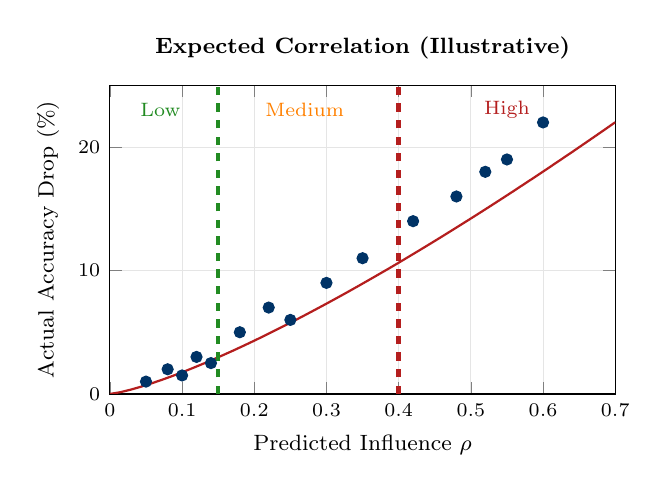
\begin{tikzpicture}
      \begin{axis}[
        width=8cm, height=5.5cm,
        xlabel={Predicted Influence $\rho$},
        ylabel={Actual Accuracy Drop (\%)},
        xmin=0, xmax=0.7,
        ymin=0, ymax=25,
        label style={font=\footnotesize},
        tick label style={font=\scriptsize},
        title={\footnotesize Expected Correlation (Illustrative)},
        title style={font=\footnotesize\bfseries},
        grid=major,
        grid style={gray!20},
      ]
        \addplot[only marks, mark=*, mark size=2pt, deepblue] coordinates {
          (0.05,1) (0.08,2) (0.10,1.5) (0.12,3) (0.14,2.5)
          (0.18,5) (0.22,7) (0.25,6) (0.30,9) (0.35,11)
          (0.42,14) (0.48,16) (0.52,18) (0.55,19) (0.60,22)
        };
        \addplot[thick, accentred, domain=0:0.7, samples=50] {35*x^1.3};

        \draw[softgreen, ultra thick, dashed] (axis cs:0.15,0) -- (axis cs:0.15,25);
        \draw[accentred, ultra thick, dashed] (axis cs:0.40,0) -- (axis cs:0.40,25);

        \node[font=\scriptsize, softgreen] at (axis cs:0.07, 23) {Low};
        \node[font=\scriptsize, orange] at (axis cs:0.27, 23) {Medium};
        \node[font=\scriptsize, accentred] at (axis cs:0.55, 23) {High};
      \end{axis}
    \end{tikzpicture}
  \end{center}
\end{frame}

\begin{frame}{Summary of Novelty}
  \begin{center}
    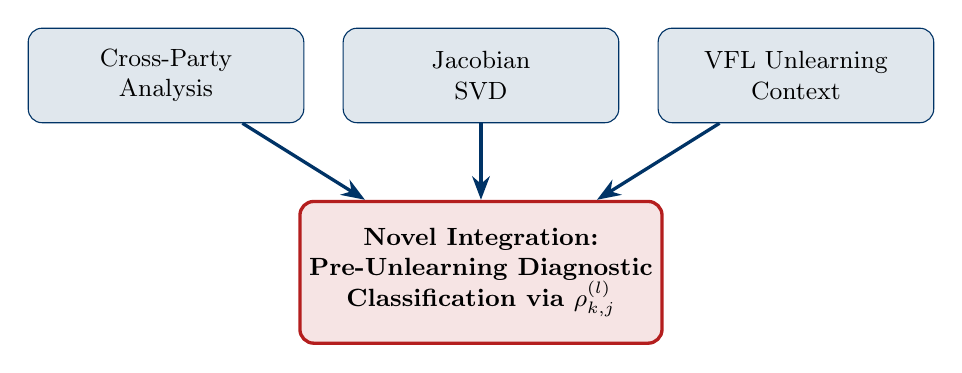
\begin{tikzpicture}[
      comp/.style={rectangle, draw=deepblue, fill=deepblue!12, rounded corners=5pt,
                   minimum width=3.5cm, minimum height=1.2cm, align=center, font=\small},
      novel/.style={rectangle, draw=accentred, fill=accentred!12, rounded corners=5pt,
                    minimum width=4.5cm, minimum height=1.8cm, align=center, font=\small\bfseries,
                    very thick},
      arr/.style={-{Stealth[length=3mm]}, very thick, deepblue}
    ]
      \node[comp] (c1) at (-4, 1.5) {Cross-Party\\Analysis};
      \node[comp] (c2) at (0, 1.5)  {Jacobian\\SVD};
      \node[comp] (c3) at (4, 1.5)  {VFL Unlearning\\Context};

      \node[novel] (ours) at (0, -1) {Novel Integration:\\Pre-Unlearning Diagnostic\\Classification via $\rho_{k,j}^{(l)}$};

      \draw[arr] (c1) -- (ours);
      \draw[arr] (c2) -- (ours);
      \draw[arr] (c3) -- (ours);
    \end{tikzpicture}
  \end{center}
  \vspace{0.3cm}
  \begin{center}
    \textit{Each component has theoretical support; the \textbf{integration} is new and fills a clear gap.}
  \end{center}
\end{frame}

% ================================================================
\section{References}
% ================================================================

\begin{frame}[allowframebreaks]{References}
  \footnotesize
  \begin{enumerate}
    \item SensFL: Privacy-Preserving Vertical Federated Learning. \textit{CMES}, 2025.
    \item Ferrari: Federated Feature Unlearning via Optimizing Feature Sensitivity. \textit{NeurIPS}, 2024.
    \item MeGU: Machine-Guided Unlearning with Target Feature Disentanglement. \textit{arXiv}, 2026.
    \item Machine Unlearning under Retain--Forget Entanglement. \textit{ICLR Submission}, 2026.
    \item S.\ Oymak et al., Generalization Guarantees for Neural Networks via Low-rank Jacobian. \textit{NeurIPS}, 2019.
    \item Wang \& Wang, Forgetting Any Data at Any Time: Certified VFL Unlearning. \textit{arXiv}, 2025.
    \item LASER-VFL: Vertical FL with Missing Features. \textit{ICLR}, 2025.
    \item Why Deep Jacobian Spectra Separate: Depth-Induced Scaling. \textit{arXiv}, 2026.
    \item Varshney et al., Unlearning Clients, Features and Samples in VFL. \textit{arXiv}, 2025.
    \item Cer-FeaUn: Certified Feature Unlearning in VFL. \textit{IEEE}, 2025.
  \end{enumerate}
\end{frame}

% ================================================================
%  THANK YOU
% ================================================================
\begin{frame}{}
  \begin{center}
    \vspace{1.5cm}
    {\Huge\bfseries\textcolor{deepblue}{Thank You}}\\[0.8cm]
    {\large Questions \& Discussion}\\[0.5cm]
    {\footnotesize Jacobian-Based Feature Entanglement Analysis for VFL Unlearning}
  \end{center}
\end{frame}

\end{document}
